\documentclass[]{report}
\usepackage{url}
\usepackage{amsmath}
\usepackage{amsmath,amssymb}
\usepackage[numbers]{natbib}
\usepackage{graphicx}
\usepackage{xcolor}
\usepackage{appendix}
\colorlet{mygray}{black!30}
\colorlet{mygreen}{green!60!blue}
\colorlet{mymauve}{red!60!blue}
\usepackage{listings}
\lstset{
	backgroundcolor=\color{gray!10},  
	basicstyle=\ttfamily,
	columns=fullflexible,
	breakatwhitespace=false,      
	breaklines=true,                
	captionpos=b,                    
	commentstyle=\color{mygreen}, 
	extendedchars=true,              
	frame=single,                   
	keepspaces=true,             
	keywordstyle=\color{blue},      
	language=c++,                 
	numbers=none,                
	numbersep=5pt,                   
	numberstyle=\tiny\color{blue}, 
	rulecolor=\color{mygray},        
	showstringspaces=false,               
	showtabs=false,                 
	stepnumber=5,                  
	stringstyle=\color{mymauve},    
	tabsize=3,                      
	title=\lstname                
}

% Title Page
\title{CM0605 - Embedded Systems Engineering}
\author{Liam Brand}
\date{}


\begin{document}
\maketitle
\tableofcontents

	\chapter{Real Time Scheduling}
		\subsection{Basic Scheduling Analysis}
			\subsubsection{(a)}
			The utilisation of a task set is given by
			
			\begin{equation}
				U = \sum_{i=1}^{N} \frac{C\textsubscript{i}}{T\textsubscript{i}}
			\end{equation}
			%equation
			
			Where N is the number of tasks, C is the task's execution time and T is the task's period. The given task set's utilization is approximately 0.99.
			
			\subsubsection{(b)}
			A set of given tasks can be proved to be or not be schedulable using rate-monotonic priority assignment by using the utilisation-bound theorem. If the test is positive and the CPU utilisation is below the given bound, the set is schedulable.
			
			\begin{equation}
			U = U = \sum_{i=1}^{N} \frac{C\textsubscript{i}}{T\textsubscript{i}} \leq n(2^\frac{1}{n} - 1)
			\end{equation}
			As previously discussed, the set's CPU utilisation is around 0.99. The given task set has 6 tasks, so the utilisation bound is around 0.73. This test is therefore false, meaning the task set is not schedulable using rate-monotonic priority assignment.
			
			\subsubsection{(c)}
			First the WCRT (worst case response time) for the task set must be calculated. This can be achieved via the given formula.
			\begin{equation}
			R_i = C_i + \sum_{j \in hp(i)} \left\lceil \frac{R_i}{T_j} \right\rceil C_j
			\end{equation}
			
			Where R is response time, C is CPU utilisation, and hp(i) denotes the set of tasks of priority higher than i.

			This calculation is repeated for each task until the calculate task response time converges twice. The following shows each iteration of this formula being applied to the task set.
			\medskip

			\textbf{Iteration 1} \newline
			E(C=14, T=48, D=48): r = 14 \newline
			C(C=6, T=240, D=240): r = 20 \newline
			A(C=42, T=330, D=60): r = 76 \newline
			D(C=132, T=360, D=300): r = 250 \newline
			B(C=72, T=720, D=660): r = 342 \newline
			F(C=18, T=4800, D=120): r = 360 \newline
	
			\textbf{Iteration 2} \newline
			E(C=14, T=48, D=48): r = 14 \newline
			C(C=6, T=240, D=240): r = 20 \newline
			A(C=42, T=330, D=60): r = 76 \newline
			D(C=132, T=360, D=300): r = 270 \newline
			B(C=72, T=720, D=660): r = 412 \newline
			F(C=18, T=4800, D=120): r = 430 \newline
	
			\textbf{Iteration 3} \newline
			E(C=14, T=48, D=48): r = 14 \newline
			C(C=6, T=240, D=240): r = 20 \newline
			A(C=42, T=330, D=60): r = 76 \newline
			D(C=132, T=360, D=300): r = 270 \newline
			B(C=72, T=720, D=660): r = 558 \newline
			F(C=18, T=4800, D=120): r = 576 \newline
	
			\textbf{Iteration 4} \newline
			E(C=14, T=48, D=48): r = 14 \newline
			C(C=6, T=240, D=240): r = 20 \newline
			A(C=42, T=330, D=60): r = 76 \newline
			D(C=132, T=360, D=300): r = 270 \newline
			B(C=72, T=720, D=660): r = 606 \newline
			F(C=18, T=4800, D=120): r = 624 \newline
	
			\textbf{Iteration 5} \newline
			E(C=14, T=48, D=48): r = 14 \newline
			C(C=6, T=240, D=240): r = 20 \newline
			A(C=42, T=330, D=60): r = 76 \newline
			D(C=132, T=360, D=300): r = 270 \newline
			B(C=72, T=720, D=660): r = 620 \newline
			F(C=18, T=4800, D=120): r = 638 \newline
	
			\textbf{Iteration 6} \newline
			E(C=14, T=48, D=48): r = 14 \newline
			C(C=6, T=240, D=240): r = 20 \newline
			A(C=42, T=330, D=60): r = 76 \newline
			D(C=132, T=360, D=300): r = 270 \newline
			B(C=72, T=720, D=660): r = 620 \newline
			F(C=18, T=4800, D=120): r = 652 \newline
	
			\textbf{Iteration 7} \newline
			E(C=14, T=48, D=48): r = 14 \newline
			C(C=6, T=240, D=240): r = 20 \newline
			A(C=42, T=330, D=60): r = 76 \newline
			D(C=132, T=360, D=300): r = 270 \newline
			B(C=72, T=720, D=660): r = 620 \newline
			F(C=18, T=4800, D=120): r = 652 \newline
			
			The final iteration shows that the task set is schedulable, as each of the task periods are less than or equal to the task response times. However, tasks A and F have a response time that exceeds their deadline, so these tasks will not meet their deadline.
			
			\subsubsection{(d)}
			The same calculations were performed as the ones in (c), but this time the tasks were organised by deadline (lowest to highest) instead of by their period. As the technique and method for calculation has already been explained and demonstrated, only the final iteration will be shown here.
			\medskip

			\textbf{Iteration 7} \newline
			E(C=14, T=48, D=48): r = 14 \newline
			A(C=42, T=330, D=60): r = 70 \newline
			F(C=18, T=4800, D=120): r = 88 \newline
			C(C=6, T=240, D=240): r = 94 \newline
			D(C=132, T=360, D=300): r = 288 \newline
			B(C=72, T=720, D=660): r = 652 \newline
		
			The final iteration shows that each task's response time satisfies the condition of being less than or equal to the task period, so the set is schedulable using deadline-monotonic fixed-priority assignment. Task A's response time is higher than its deadline however, so it will not meet its deadline.
			
			\subsubsection{(e)}
			Files are an example of a mutual exclusive resource, as only one task can be accessing a file at any given time to perform read or write operations on it. Another example is components like hardware timers, as if multiple tasks want to use the timer there will need to be controlled access to it. 
			\medskip

			\textbf{Priority Inversion}\newline
			An example which exhibits priority inversion can be seen with the Mars Pathfinder. The Pathfinder spacecraft has an information bus which was used to exchange information between the robot's various components. A high priority task ran frequently to manage the data on this bus, and access to the bus was synchronised with a mutex. The Pathfinder had another task for gathering meteorological data, which ran infrequently and had a low priority.  This task would acquire the bus' mutex before writing data to the bus. If an interrupt caused the information bus to be scheduled whilst the meteorologic task held it, the bus management task would pend on the mutex and wait for the meteorologic task to be done.  There was also a task with medium priority that dealt with communications. 
			
			The problem with priority inversion manifested like so. An interrupt would sometimes occur that scheduled the medium priority communications thread to be scheduled during the small moments where the high priority bus thread was blocked waiting on the meteorological data thread. When this happened, the communications task would prevent the meteorological task from running which would in turn prevent the communication task from running, meaning the medium priority task was essentially blocking the high priority task\cite{jones1997really}.
			\medskip
			
			\textbf{Priority Inheritance}\newline
			Priority inheritance can help prevent this. With priority inheritance, tasks that block higher priority tasks will inherit the higher task's priority for the duration of the blocking. Once the task has finished executing and has released the resource it will drop down to its original priority asignment, and allow the high-priority task to use the resource that it has just acquired. For the Pathfinder example, this would mean the meteorologic thread would escalate to the bus management task's priority meaning the communication's task could not acquire the mutex and block the bus management task once the meteorological task had finished executing. 
			\medskip
			
			\textbf{Priority Inheritance Limitations}\newline
			Transitive blocking can occur. This is when tasks all begin blocking eachother and acquire high importance. For example, there are three tasks with high, medium and low priority, and two resources called R1 and R2. The low task takes R1 and the medium task takes R2. If the medium task wants to take R1, it is blocked and the low tas's priority is set to medium. If the high task then wants to take R2, it is blocked and sets the medium task to high priority. The task holding R1 has an unchanged priority here even though it is the reason the original high priority task is being blocked.
			
			Priority inheritance also does not prevent deadlocks, where all tasks aer stuck waiting for other tasks to release resources preventing them from releasing resources that other tasks need and so on.
			
			As well, priority inheritance might prevent priority inversion but it doesn't minimize the time that tasks spend being blocked.
			\medskip
			
			\textbf{An Alternative}
			To counter these problems, the priority ceiling protocol can be used. This involves assigning resources a priority ceiling, which is a priority that is equivalent to the highest priority of a task that is able to acquire the resource. This improves basic priority inheritance by minimizing the duration of blocking to, at most, the duration of a single critical section of a lower priority task\cite{goodenough1988priority}.
		
		\subsection{Scheduling with Shared Resources}
			\subsubsection{Question a}
			The utilisation bounds theorem requires knowledge of exact task statistics such as the task periods and deadlines, and this cannot be guaranteed for every task that needs to be tested. As well, the theorem represents a utilisation value indicative of all tasks in a set starting simultaneously (e.g. at time t = 0), making it incredibly pessimistic. A better formula would determine the schedulability of a task set as a function of individual task CPU utilisations\cite{bini2001hyperbolic}. The formula that does this is the hyperbolic bound formula, and can be seen at \ref{hyperbolicbound}.
			
			\begin{equation}
			\label{hyperbolicbound}
			\prod_{i = 1}^{n}(U\textsubscript{i} + 1) \leq 2
			\end{equation}

			\subsubsection{Question b}
			Fig \ref{fig:tasktimeline} shows the task timeline and the timeline key.
			\begin{figure}[h!]
				\centering
				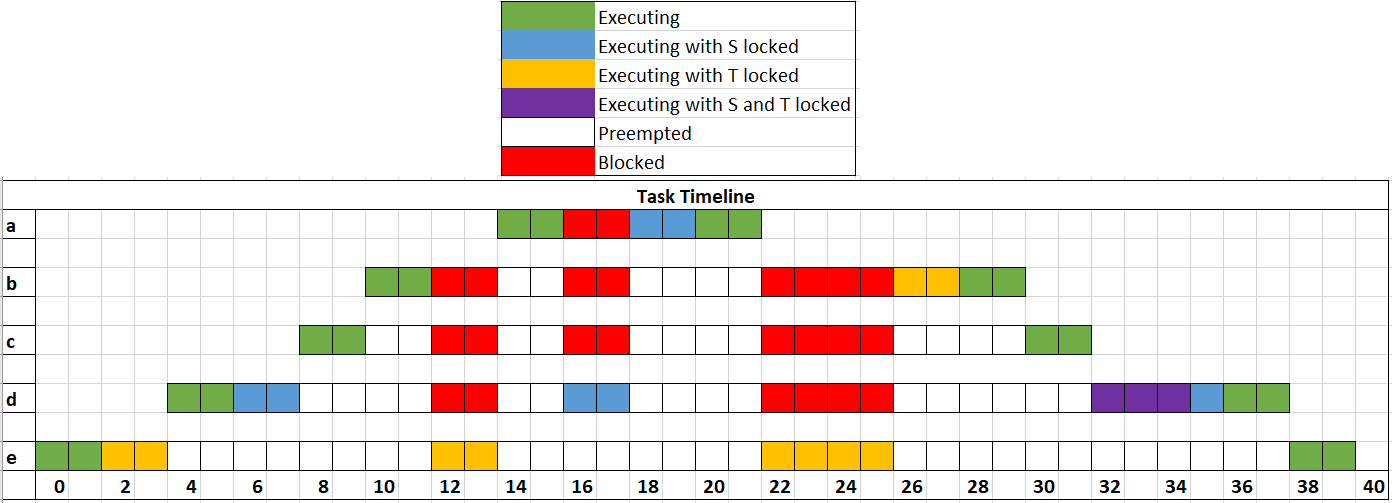
\includegraphics[scale=0.3]{tasktimeline.png}
				\caption{Task Timeline}
				\label{fig:tasktimeline}
			\end{figure}
			\newline
			\textbf{Tick 12} - Task E possesses Resource T, so it inherits the priority of Task B which attempted to acquire it and was subsequently blocked. \newline
			\textbf{Tick 13} - Task A with a priority higher than Task B (and therefore E as it has inherited B's priority) begins. \newline
			\textbf{Tick 16} - Task A attempts to acquire Resource S which Task D currently has locked, so Task D inherits Task A's priority. \newline
			\textbf{Tick 18} - Task D finishes its execution with Resource S, so the resource is released and the Task returns to its original priority. Task A can now continue executing. \newline
			\textbf{Tick 22} - Task A finishes so Task B attempts to continue executing, but when it attempts to acquire Resource T which Task E holds, it is blocked. Task E inherits B's priority and executes, blocking all other tasks as it now possesses a higher priority. \newline
			\textbf{Tick 26} - Task E finishes with Resource T, releases it and moves down to its original priority. From here, execution continues in a normal fashion according to priority. \newline
	
	\chapter{A Distributed Real-time System}
		\section{Question 1}
		For both systems, the CAN controller was initialised with a baud rate of 125000. The Display system would be event driven, responding to interrupts generated by events. The engine monitor would be a time-triggered system, with the interrupts being generated from a timer.
			
			\subsection{Display}
			For the Display system, two threads are used. These threads are assigned priorities and tasks for them to run, with one thread running the request task and the other running the display task. Of the two threads one of them had to have a slightly priority. The request thread was chosen for this as it was deemed important that it was regularly able to request information from the EngineMonitor, more so than the ability to display it. 
			
			The request thread uses a wait command to run at intervals of 500ms, and transmits a simple CAN message requesting a temperature reading to the EngineMonitor each time it runs. The message is a canMessage\_t struct, a simple structure containing variables like the message's ID, its length and some data.
			
			The full request task can be seen below.
			
\begin{lstlisting}
static void requestTask(void) {
	static canMessage_t requestMsg = {0x23, 8, 0, 0};
	bool txOk;
				
	while(true) {
		txOk = canWrite(&requestMsg);
		wait_ms(500);
	}
}
\end{lstlisting}			
			One aspect in particular that took some planning was allowing the display task to be event driven. Rather than running at an interval it had to execute and display a value to the terminal whenever it was received a temperature reading.
			
			To achieve this a combination of an interrupt handler and a semaphore is used. The display task pends on a semaphore that is released by a method that runs when a CAN message is received.
			
\begin{lstlisting}
/* A simple interrupt handler for CAN message reception */
void canHandler(void) {
	canTransferRxFrame(&rxMsg);
	rxDone.release();
}
\end{lstlisting}

			This interrupt handler transfers the most recently received CAN rxFrame to the rxMsg variable, and then releases the semaphore that the display task is pending on. Once the semaphore is released, the rest of the display code runs where it prints the data from the received message to a terminal. After the wait period has elapsed, it begins and pends on the semaphore once again. The full display task code can be seen below.
			
\begin{lstlisting}
/* Pend on a semaphore released by an RX Interrupt
* When released, display the recieved temperature reading to a terminal
*/
static void displayTask(void) {
	canRxInterrupt(canHandler);
	while(true) {
		rxDone.wait();
		pc.printf("Temperature: 0x%08lx\n", rxMsg.dataB);
	}
}
\end{lstlisting}

			\subsection{EngineMonitor}
			The EngineMonitor consists of two tasks. A tacho task which simulates monitoring the engine's rotation speed, and a temperature task which sends a response to the Display's request for a temperature reading. A time triggered scheduler is used to run the EngineMonitor tasks. 
			
			The scheduler is relatively simple, it uses a task table containing an array of task control blocks. Each block has a pointer to the task, a delay, and a period. The scheduler initializes by iterating through the task table and setting all values to zero, and all task pointer to NULL. Tasks are added to the scheduler by through the schAddTask method, which takes parameters corresponding to the variables in the task control blocks. The scheduler is then started, which begins a simple timer that starts ticking. The scheduler is then dispatched each tick, running tasks that delays have reached zero and resetting the delay's to the task's period. 
			
			The code in the EngineMonitor's main method that intialises the timer, adds the temperature and tacho tasks, then starts and repeatedly dispatches the timer can be seen below.
			
\begin{lstlisting}
schInit();
schAddTask(tachoT, 0, 20);
schAddTask(tempT, 0, 500);
			
schStart();

while (true) {
	schDispatch();
}
\end{lstlisting}

			The tacho task simulates measuring the engine's rotation speed by reading some values from the K64F's accelerometer, and assigning these values to a dummy variable which isn't used anywhere else in the program.
			
			When the temperature task runs, it waits on the canReady method returning true. canReady is a simple method that returns true if there is data ready to be read from the CAN port. If the method returns true, the task uses canRead to read the message into a canMessage\_t variable.
\begin{lstlisting}
if(canReady()){
	canRead(&canData);
	id = canData.id;
}
\end{lstlisting}

			Following this, the message's id is checked. Rather than simply responding once any message is received, an id of 0x24 is used for all request messages, and should the received message match this id it will be acknowledged as originating from the display. Once this acknowledgment has been done, values are collected from the accelerometer to simulate taking a temperature reading, they are put into a can message, and the message is then written to the CAN controller.	
\begin{lstlisting}
if(id == 0x24){
	canMessage_t txMsg = {0x23, 8, acc.getY(raY), acc.getY(raY)};
	bool txOk;
	pc.printf("ID 0x%1x", canData.id);
	txOk = canWrite(&txMsg);
}
\end{lstlisting} 

		\subsection{System Evaluation}
		The system's structure and timing requirements have been fulfilled. Both the display and engine monitor systems posses the correct structure, in that they have appropriate tasks that perform the desired functions, and the tasks in both run in their respectively specified event driven and time-triggered ways. The tasks also run at their specified time periods, with the request task running ever 500ms and the tacho task running every 20ms. The temp task only runs in response to a request, and the request it receives is checked before a response is sent rather than simply sending a request as soon as any message is received.
		
		This structure affords them some degree of precision. Both systems could achieve their functionality with a super-loop, with large looping main tasks that perform certain functionalities each loop. The problem with this would be in its lack of precision and efficiency however. By using an event driven system for the display, it can be ensured that the display responds to an event as soon as it is received rather than an event occurring and then the potential for a small wasted interval to occur whilst it loops back around to the relevant code. With the engine monitor, a time triggered system helps ensure that tasks run closer to their correct time, as in a super loop there's no guarantee that all other code in the loop will take the same amount of time to execute each loop. The system being set up the way it is helps minimize the intervals between necessary functionality.
		
		\medskip
		
		The system has no functionality in place to deal with a message that hasn't successfully been sent however. The canWrite method returns a boolean value depending on whether or not the message has been successfully sent (true if it has, false if it hasn't), and this value is never used for anything. The system could be improved by checking this value once the canRead method is called, and if it returns false it could begin a retry loop where it attempts to send the message again. This loop would continue until the next time the task this is in has to run (e.g. until the next new request message needs to be sent from the display), and should the message never be sent this could flag up as a missed message. Repeated missed messages could be flagged up as a more serious problem. As of right now, the system is massively dependent on all messages successfully sending, with no warning of requests or temperature acknowledgements that haven't been able to be sent.
		
		The display system also performs all display functionality in the interrupt service routine. Whilst this doesn't seem to have any adverse effects yet, should the system expand and begin doing something more elaborate with received temperature data such as printing to an attached LCD, doing everything in the ISR might start to impede performance. To help with this, an EventQueue could be used. The Mbed RTOS features an EventQueue API\cite{mbedoseventqueue} that can be used to store events and defer the execution of the event code for a different context. For the display's ISR, the EventQueue could store interrupts containing temperature values and execute them outside of the interrupt context to prevent the interrupt blocking other tasks for too long.
		
		\section{Question 2}
			\subsection{Measurement Procedure}
			The FRDM-K64F features programmable interval timer chips, which have been employed here to measure the execution time of code. By starting and stopping a PIT and retrieving the elapsed cycles, the amount of time that has elapsed during the execution of code can be measured. This is how the computation times of the temp and tacho tasks were performed. 
			\medskip
			
			Before measurement, the counters were started and then instantly stopped. This was done to determine the amount of clock cycles it took to begin and end the counter, this could be subtracted from any measurements to gain a more accurate reading. Once this was done and saved as an entropy value, the PIT was started before the execution of a task in question and stopped after its code had finished executing. The entropy was then subtracted from this measurement. These measurements were taken over the course of a few minutes of the program running, and and an average, best, and worst computation time were recorded over the course of around 500 individual readings. The below code snippet shows this process being used to measure the tacho task.
			\begin{lstlisting}
	void tachoT(void){
		counterStart();
		int16_t dummyx = acc.getY(raY);
		timeElapsed = counterStop() - entropy;
			
			
		if(timeElapsed < bestTime){
			bestTime = timeElapsed;
		}
			
		if(timeElapsed > worstTime){
			worstTime = timeElapsed;
		}		
	}
			\end{lstlisting}
			
			\subsection{Measurement Quality}
			The clock cycle measurements here should be fairly high in precision, as an average will help factor out noise from other readings and the time triggered nature of the engine monitor means that any interrupts will happen on a regular enough basis to not cause sporadically high or low readings.
			\medskip
			
			% is this right?
			In terms of accuracy, the removal of the entropy should help somewhat. The timer interrupts will affect the readings here though. The temperature task runs at a period of 500, and the tacho task runs at a period of 25. This means that the tacho task should run around 25 times between each run of the temperature task, and these executions will affect the measurement of the temperature task's execution as the tacho task will be generating interrupts and blocking the task. This will be less of a problem for the tacho task with how frequently it runs, whilst there will be occassions where the interval is close and the tacho task is blocked by the temperature task, this will be infrequent enough for the average reading to reduce its impact. 
			
			Timing jitter is also a consideration here, where things like electromagnetic interference will affect the resulting clock cycle value by adding noise to it. The average should help somewhat here too, as the noise won't always be exactly the same and the average should help factor out more significantly noisy readings. The best case and worst case readings however aren't averaged out, so they could be affected significantly as they might just be a result of the least and most noise rather than true code execution time.
			
			500 iterations isn't a massive amount either, as it only accounts for a few minutes of system activity. A more accurate understanding of the execution time could be gained if these measurements were taken over the period of a few hours.
			
			\subsection{Worst-Case Time}
			The measurements for the temperature task can be seen in \ref{executionmeasurementstemp}.
			
			\begin{table}[h]
				\centering
				\begin{tabular}{| l | l | l |} 
					\hline
					Reading & Cycles & Real-Time ($\mu $s) \\ [0.5ex] 
					\hline
					Average  & 16771 & 139.75 \\ 
					Best & 16763 & 139.69 \\
					Worst & 16931 & 141.09 \\
					\hline
				\end{tabular}
				\caption{Temperature Task Readings}
				\label{executionmeasurementstemp}
			\end{table}
		
			The measurements for the tacho task can be seen in \ref{executionmeasurementstacho}.
			
			\begin{table}[h]
				\centering
				\begin{tabular}{| l | l | l |} 
					\hline
					Reading & Cycles & Real-Time ($\mu $s) \\ [0.5ex] 
					\hline
					Average  & 8333 & 69.44 \\ 
					Best & 8328 & 69.4 \\
					Worst & 8342 & 69.51 \\
					\hline
				\end{tabular}
				\caption{Tacho Task Readings}
				\label{executionmeasurementstacho}
			\end{table}
		
			The worst-case execution scenario is the following. The request from the display arrives just as the temperature task has finished an execution, so the task period of 500ms needs to elapse before it will run again. Once this is about to elapse, the tacho task is then scheduled to run just before. Once this has finished its execution, the temperature task finally runs and processes the request.
			
			The worst case execution time then can be represented by the temperature task's period, the tacho task's worst measured computation time and the temperature task's worst execution time. This is 500ms + 69.51$\mu s$ + 141.09$\mu s$, giving a worst case execution time of 500.2106 milliseconds.
		
			%The worst-case execution time would be achieved with the arrival of a request right as the temperature task has finished executing. For the request to be read here, the period between temperature task executions will need to elapse and then the temperature task will run. Therefore, the worst case execution time is the 
			
			%and just before the tacho task begins its %execution. For the request to be read here, the tacho task would need to complete its execution, the interval between temperature task executions would need to be waited for, and then the temperature task would need to be execute. We can find this by adding the worst measurements from both the temperature and tacho task, which comes to around 210.6 microseconds.
			
			\subsection{Time-Triggered and RTOS - Response Times}
			Time-triggered schedulers can have a negative effect on responses due to their static response schedule. When an event is received, there will be a period of time where the system is waiting for the necessary response task to run and respond to it. This is contrasted to a real time system's capability for a much more immediate response to events. Albert et al\cite{albert2004comparison} demonstrates this in the test scenario comparing a time and event driven system during a critical situation. As well, it's noted that because transmission cannot take place until the response has ran and the time at which a critical situation will occur isn't known, the response period for a time-triggered system is susceptible to jitter as there's no way of knowing where tasks will be in their executions or delay periods when the critical event arrives.
			
			\subsection{Time-Triggered and RTOS - Wider Evaluation}
			As previously discussed, an RTOS will allow for faster response times in comparison to a time-triggered system. This is a significant advantage in ensuring that a system is able to react to critical events as quickly as possible, but care must be taken to ensure that the system doesn't get overwhelmed. Kopetz\cite{kopetz1991event} discusses the occurance of \textit{C-events}, chance events that cannot be properly predicted. In the discussion it's noted that since a computer system only has a finite amount of resources, all received chance events cannot be processed. This requires the implementation of measures to deal with these "event showers" by ensuring that the flow of information to the system is restricted to prevent it buckling under the weight of the events, but also that these events are still stored to prevent any of them being discarded and not being dealt with. Whilst the lack of timing specification can provide flexibility in dealing with events, Lee\cite{Lee:EECS-2009-30} notes that the timing becomes increasingly uncontrollable and unpredictable as RTOSs grow in complexity. More inter-process communication introduces more factors that have an effect on the program flow like interrupts, additional priorities and the need for more things like locks. This can make program quality worse as obscure timing bugs that only occur very rarely might not be predicted and may not show themselves during testing, and the brittle nature of the timing means small system changes could have large unforeseen impacts.
			
			A real time operating system then can provide a system capable of rapid-response to events, making it a potentially good choice for safety-critical and mission-critical systems given their potential for severe consequences if problems aren't addressed quickly enough. Care needs to be taken during implementation however to ensure that the system is capable of dealing with large quantities of events without failing, and that the system is also designed properly to help ensure its predictability and robustness.
			\medskip
			
			In their discussion of the time-triggered architecture, Kopetz and Baeur\cite{kopetz2003time} mention how it simplifies large embedded applications through its decomposition of the system into simple nodes. The global time used to execute tasks allows a more exact specification of when and how tasks should be run, and also guarantees the "timeliness of real-time applications". This precision and predetermined assignment of task intervals offers some simplicity in the program's initial design, and the scheduled execution of tasks and response to events helps prevent a large influx of events causing problems as it might do in a real time system. As previously mentioned however, this has the downside of a potentially worse response time to these events, which in a safety or mission-critical system could have massive consequences. Whilst this does make a time-triggered scheduler potentially worse for mission-critical or safety-critical systems, smaller systems with less severe consequences in the event of a fault might benefit from the time-triggered architectures simplicity and predictability. As well, a system with more predictable faults whose occurrences can be accurately predetermined may fare well better with a time-triggered scheduler, as it is significantly easier to ensure that created tasks meet their imposed deadlines.
		
		\section{Question 3}
		The formula for calculating the CAN message response time is shown in \ref{canmessageresponse}.
		
		\begin{equation}
		\label{canmessageresponse}
		R\textsubscript{m} = J\textsubscript{m} + w\textsubscript{m} + C\textsubscript{m}
		\end{equation}
		Where J is queuing jitter, w is worst-case queuing delay, C is worst-case message transmission time and \textsubscript{m} is the message. This question assumes no queuing jitter, so the final formula used to calculate the message response time here will only involve w and C.
		\medskip
		
		The message's worst-case transmission time can be calculated using \ref{worstcasetransmission}.
		\begin{equation}
		\label{worstcasetransmission}
		C\textsubscript{m} = (g + 8s\textsubscript{m} + 13 + \lfloor \frac{g + 8s\textsubscript{m} - 1}{4} \rfloor ) \tau bit
		\end{equation}
		
		Where g is 34 for a standard CAN frame, s\textsubscript{m} is the number of data bytes in the message, and \textsubscript{$\tau bit$} is the transmission time for 1 bit. This formula is simplified to \ref{worstcasesimplified} for 11 bit identifiers, which is what the CAN devices being employed here use.
		
		\begin{equation}
		\label{worstcasesimplified}
		C\textsubscript{m} = (55 + 10s\textsubscript{m})\tau bit
		\end{equation}
		
		The CAN messages being sent in the system are 8 bytes long, and the controllers use a baud rate of 125000 meaning they send 125000 bits in one second. From this, 1/125000 can be used to determine a single bit is transmitted in 0.000008 seconds, which is 8 microseconds. The formula in \ref{worstcasesimplified} can now incorporate these values.
		\begin{equation}
		\label{worstcasesimplifiedrealnumbers}
		C\textsubscript{m} = (55 + 80)8 = 1080
		\end{equation}
		\medskip
		
		Now the worst-case transmission time is understood as 1080 microseconds. This number is multiplied by two because the response procedure involves the transmission of two messages, the request message and the acknowledgement message. This gives a worst-case transmission time of 2160.  Now the worst-case queuing delay needs to be calculated using the formula in \ref{queue}.
		
		\begin{equation}
		\label{queue}
		w\textsubscript{m} = B\textsuperscript{MAX} + \sum_{\forall k \in hp(m)}{\lceil \frac{w\textsubscript{m} + J\textsubscript{k} + \tau bit}{T\textsubscript{k}} \rceil}
		\end{equation}
		
		Where B\textsuperscript{MAX} is the longest possible transmission time of a message on the bus, hp(m) is the set of all messages with a higher priority than message m, and T is the task period.
		
		\section{Question 4}
		Predictability in terms of an embedded control system concerns prior knowledge of a program's behaviour. Henzinger\cite{henzinger2008two} defines predictability for embedded software design as a number of different factors. These are the program's functional properties (e.g. what output does the program compute?), its reaction properties (e.g. when does the program provide the output?) and the program's execution properties (e.g. what resources are consumed to provide this output?). Lee\cite{Lee:EECS-2009-30} gives a similar explanation, in that predictable behaviour is program behaviour that can be determined in finite time through analysis of the program's design. Given information about the program's design, its behaviour should be able to be inferred depending on what inputs the program is given.
		\medskip
		
		With regards to predictability in a sound engineering approach, one of the biggest reasons it allowing a good prediction of system performance over a large timeframe. Stankovic and Ramamritham\cite{Stankovic93whatis} discuss this, saying that a predictable system's overall performance and the performance its individual tasks are easy to ascertain with any complex evaluation. As well, they talk about how a predictable system offers a clearer indication of whether or not the system's tasks will meet their imposed deadlines. From this, it can be easily ascertained whether or not the timing requirements on more critical tasks can be met over a long time span. 
		
		Feiler et al\cite{feiler2000improving} discuss the system's performance over a timeframe aspect in a bit more detail. Predictability doesn't just help in understanding a system's viability for operation in the immediate future, but for the incredibly long life span that some systems posses. For example in fielded systems such as mission-critical military or aviation systems, systems will not be completely redesigned from the ground up every time a new piece of technology is made. Often existing systems are simply upgraded, specifically the hardware. As hardware becomes obsolete these systems may be moved over to something else, and a lack of system predictability makes the consequences of these actions difficult to foresee. This could result in impacts on the system's performance or reliability that occur during operation. For a less critical system this might have the drawback of some downtime, for a more critical system such as something in aviation this could lead to consequences far more catastrophic.  As well, poorly understood resource consumption can incur a significant financial cost as more money will need to be spent on integration, maintenance and hardware upgrades. Even once this has been done, there is no guarantee that more changes won't be needed as the system's lack of predictability could mean there are faults present that simply haven't manifested themselves yet.
		
		As mentioned in the discussion of RTOSs previously, a real time operating system can grow to be incredibly complex and this can give it an element of unpredictability. If a system's behaviour is more predictable, the system will be easier to test as there is a significantly lower chance of obscure bugs occuring due to unforeseen system events.
	
	\chapter{Reliability}
		\section{Section 1}
			\subsection{(a)}
				\subsubsection{Fail-Operational}
				Fail-operational is when a system is still capable of full performance in the presence of faults, with no external signs of the fault manifesting. For the car production line, this would mean a system fault would still result in cars being produced at a good efficiency, meaning the system's objectives to produce cars won't be impeded and as such neither will car production. The encountered fault might cause an issue where damage is done to cars however, so whilst the production might not fail the actual quality of the cars produced would. As well, there would be no guarantee for the system to be entirely safe during its operation here, so there would be a risk to personnel safety.
				
				\subsubsection{Fail-Active}
				Fail-active systems can continue their operation when a fault is encountered, but will do so at a reduced performance. This is 'graceful degradation' where as more parts of the system experience faults the system can still continue its operation (up until a certain point). With regards to the production line, this will likely involve car production continuing at a reduced rate until the fault can be corrected. This won't always be the case however, as the fault may lie in a specific part of the car assembly. If this was the case, reduced system performance isn't tolerable as a key part of the manufacturing process won't be completed, so the cars being produced here won't be of any use.
				
				\subsubsection{Fail-Safe}
				Fail-safe systems will cease operation upon encountering a fault, and enter a safe mode. For example, elevators are often equipped with breaks that will apply should the cable holding the elevator snap. For the car production line, this will mean the entire system ceases operation in the event of a fault. This will completely minimize risk to human life but production will suffer the most as each encountered fault will result in the system entering its safe mode. Restarting the system and bringing it back to full operational capacity could take a while, and this will result in a potential failure of the system's mission objectives.
				
				\subsubsection{High Availability}
				High availability systems cease operation upon encountering a fault, but must be returned to operation as quick as possible, this can involve hot swapping system units whilst the system is operating. These systems allow for failures, and aim to achieve a high mean time of operation rather than a long continuous time of operation. The goal here is not to avoid faults, but to minimize time spent rectifying them so that the overall system operation time is as high as possible\cite{gray1991high}. The availability of these system can be measured by the following, where MTBF is mean time between failures and MTTR is mean time to repair.
				\begin{equation*}
				Availability = MTBF/(MTBF + MTTR)
				\end{equation*}
				
				Out of the different types of fault-tolerance, high-availability would be the most appropriate for the car assembly line. Whilst this will result in a lower amount of continuous operation time, as long as the mean operation is as high as possible (which high-availability aims to achieve) production goals should still be satisfied and the production line's mission shouldn't be impeded. High-availability also allows for shutdowns when faults are encountered, which is an imperative feature of the assembly line's fault tolerance given the potential for harm to personnel.
			
			\subsection{(b)}
				\subsubsection{Potential Risks}
				The nature of the car assembly line means any single failure will cause the entire system to fail, so in terms of the network only a single connected node in the distributed system needs to experience a problem for the entire system to stop working. 
				
				Timing will also be essential within the assembly line to ensure the robotic tools perform their jobs properly, so there is a risk of performance overhead negatively impacting the system too. Networked processors that are in close proximity will communicate incredibly quickly, but processors that are further away from the network will take longer to communicate and this will need to be accounted for otherwise tools may not behave as expected and, should any issues occur, the entire system will fail as previously discussed. In a similar vain, timing will need to be considered to ensure that all operations across the network are in synchronisation with each other. Messages arriving on time is a good start, but this doesn't guarantee that all of the production line robotics are cooperating as expected.
				
				As well, there is the simple nature of hardware failure to contend with. Individual components on the production line could experience failure, and if one component fails then production will have to cease until it can be repaired. Connected nodes on the network might experience hardware faults as well, with nodes either failing or experiencing problems that cause data corruption. The nodes could also experience addressing errors where nodes send or receive messages intended for other nodes, causing problems with system synchronisation. Faults with the sensors could also cause shutdowns, with sensors giving erroneous readings or being inaccurate due to a high amount of noise causing inaccurate readings.
				
				\subsubsection{Architecture Recommendation}
				Redundant systems could be used to minimize the impact of faults. Essential hardware components such as power supplies for the production line's robotics could be utilized so that if they fail backup components can safely continue operation, preventing a drop in production but also avoiding any risk to personnel. For the sensors, n-version programming could be used to counter the effects of noise and sensor hardware faults. A checking system could be used that compares sensor values and settles on an overall average, with sensor values that are abnormal in comparison to all other values being selectively ignored. This would help prevent erroneous readings from causing shutdowns, but the voter system would ensure that should many sensors produce abnormal readings a genuine problem can still be detected.
						
			
			\subsection{(c)}
			Power-on risks with the production line's hardware will need to be considered. The component's ROM contents could become corrupted by electromagnetic pulses, or the component's flash memory could be reprogrammed and cause issues (e.g. maybe parts of the memory are being incorrectly erased). These issues can be solved during the component's power-up phase by having the component run checks to ensure the validity of its state.
			\medskip
			
			Run-time issues are also a possibility. Like with the start up problem, electrical noise or a power supply fluctuation could cause the program the component is running to become corrupted. Check summing could be used here, where the component's program checks its validity against a checksum to determine if the program is in a proper state. Program copies could be used that have also been check summed, with components running the check summed copies should the program running be found to be corrupt.

		\section{Section 2}
			\subsection{(a)}
				\subsubsection{Regular Sensor}
				\textbf{Number of Outputs} - 240 \newline
				\textbf{Maximum Absolute Discrepancy} - 13.4 \newline
				\textbf{Mean} - 102.09 \newline
				\textbf{Standard Deviation} - 6.37 \newline
				
				\subsubsection{Faulty Sensor}
				\textbf{Number of Outputs} - 242 \newline
				\textbf{Maximum Absolute Discrepancy} - 104.0 \newline
				\textbf{Mean} - 121.80 \newline
				\textbf{Standard Deviation} - 36.22 \newline
			
			
			\subsection{(b)}
				For each of the sensor setups, the last three readings are shown.
				\subsubsection{1 Faulty, 2 Non-Faulty}
					\begin{table}[h!]
						\begin{tabular}{| l | l | l | l | l |}
							\hline
							Reading & Nominal Value & Deviation & Mean   & Standard Deviation \\
							\hline
							98.70   & 102.0         & -3.3      & 101.19 & 13.14              \\
							107.33  & 103.0         & 4.3       & 101.22 & 13.11              \\
							101.75  & 102.0         & -0.3      & 101.22 & 13.09        	\\
							\hline      
						\end{tabular}
					\end{table}			
			
				\subsubsection{1 Faulty, 3 Non-Faulty}
					\begin{table}[h!]
						\begin{tabular}{| l | l | l | l | l |}
							\hline
							Reading & Nominal Value & Deviation & Mean   & Standard Deviation \\
							\hline
							99.35   & 98.0          & 1.3       & 107.45 & 15.75              \\
							99.02   & 97.0          & 2.0       & 107.42 & 15.73              \\
							96.05   & 98.0          & -1.9      & 107.37 & 15.71              \\
							\hline
						\end{tabular}
					\end{table}
				
				The Simulation class was invoked from the command line with 100 and 5 for the nominal and noise values respectively. The program was modified to take two additional parameters, one for the amount of regular sensors and one for the amount of faulty sensors, and the appropriate number of these sensors was input depending on which of the two tests were being performed. Faulty sensors were initialised with with a fault interval of 10000 milliseconds and a fault value of 200. Code can be viewed at Appendix \ref{sensorsimcode}.
				
			\subsection{(c)}
			
			
		
	\bibliographystyle{plainnat}
	\bibliography{papers}
	\newpage
	\begin{appendices}
	\chapter{SensorSim Array}
	\label{sensorsimcode}
	\lstinputlisting[caption=Simulation.java, language=java, showstringspaces=false]{arraySim.java}
	\end{appendices}

\end{document}          
